\chapter{Analise Léxica}\label{fund}
Neste capítulo será descrito a base de conhecimento utilizada para o desenvolvimento do analisador léxico, assim como a importância desta fase dentro do projeto.
\section{O papel do analisador léxico}\label{label1}
A fase de análise léxica tem como objetivo identificar e separar em \textit{tokens}, trechos do código fonte em um padrão definido de acordo com linguagem do fonte.\par
Esta fase é responsável por ler os caracteres do código fonte agrupando-os em um fluxo de \textit{token}, onde cada \textit{token} representa uma serie de caracteres que possua um sentido lógico, como por exemplo, a identificação de uma palavra reservada da linguagem utilizada (if, while e etc), ou até mesmo um caractere de pontuação ou uma operação composta por mais de um caractere (==, \&\&, ; e etc).
Esta série de caracteres que formam um \textit{token} é chamada de lexema para aquele \textit{token}.\par
A identificação destes \textit{tokens} será de importância para complementar junto a analise sintática a construção da estrutura de uma arvore sintática, que será abordada nos capítulos subsequentes. Estrutura essa responsável por auxiliar na representação ao usuário, da ordem em que cada ação dentro do fonte será executada.\par
Estes \textit{token} gerados serão utilizados para identificar as regras de produção de expressões lógicas da linguagem.
Este analisador será construído para a linguagem C, afim de identificar algoritmos determinísticos. Isto é possível, dado que a linguagem C é uma linguagem livre de contexto, pois possui uma gramática simplificada.


\begin{citacao}
``Uma gramática descreve naturalmente a estrutura hierárquica de muitas construções das linguagens de programação. Por exemplo, um comando if-else, em C, possui a forma
if(expressão) comando else comando
Ou seja, o comando é uma concatenação da palavra-chave if, um parêntese à esquerda, uma expressão, um parêntese à direita, um comando, a palavra-chave else e um outro comando. Usando-se a variável expr a fim de denotar uma expressão a variável cmd para um comando (ou enunciado), esta regra de estruturação pode ser expressa como 
cmd -> if(expr) cmd else cmd
Onde seta pode ser lida como "pode ter a forma". Tal regra é chamada de produção. Numa produção, os elementos léxicos,
Como a palavra-chave if e os parênteses, são chamados de tokens. 
As Variáveis como expr e cmd representam sequências de tokens e são chamadas de não terminais.'' Pag 12 livro do dragão \cite{wang}
\end{citacao}

\begin{figure}[htp!]
\centering
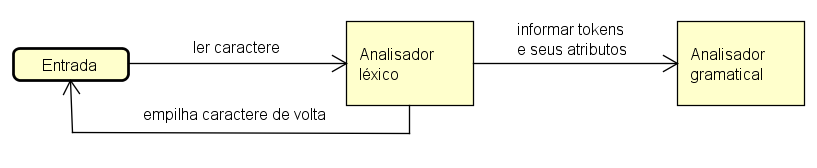
\includegraphics[width=\textwidth]{figuras/flxlexico.png}
\caption{Fluxo processual da análise léxica}
\label{figura1}
\end{figure}

\section{Especificação de tokens}\label{labelS1}
Expressões regulares são uma forma de especificar padrões. Cada padrão é correspondente ao respectivo conjunto de cadeias. Assim as expressões regulares serão responsáveis por um conjunto de cadeias de caracteres.
\par Uma expressão regular trata-se de uma notação que irá representar uma determinada sequência de caracteres. Este tipo de notação é empiricamente utilizado para validar entrada de dados ou fazer buscas e extração de informações em formato de texto.
\par Dentro da sintaxe de expressões regulares existem metacaracteres que podem ser classificados em quatro conjuntos:

\begin{itemize}
\item  Especificadores: determinam uma cadeia de caracteres a ser encontrada em uma determinada posição.
\item Quantificadores:  definem a quantidade de vezes que determinada sequência de caracteres irá se repetir.
\item Âncoras: Estabelecem a posição que determinada expressão irá ocorrer.
\item Agrupamento: Definem grupos ou alternativas possíveis.
\end{itemize}

\begin{table}[htbp!]
  \centering
    \caption{Especificadores}
      \begin{tabularx}{\textwidth}{|X|X|X|}
      \hline
      \textbf{metacaractere} &  \textbf{alcunha} & \textbf{significado} \\
      \hline
      . & curinga & qualquer caractere, exceto a quebra de linha. \\
      \hline
      [...] & conjunto & qualquer caractere incluído no conjunto.\\
      \hline
      [\textasciicircum{}...] & conjunto negado & qualquer caractere não incluído no conjunto.\\
      \hline
      \textbackslash{}d & dígito & o mesmo que [0-9]. \\
      \hline
      \textbackslash{}D & não-digito & o mesmo que [\textasciicircum{}0-9]. \\
      \hline
      \textbackslash{}s & branco & espaço, quebra de linha, tabs etc.; o mesmo que [\textbackslash{}t\textbackslash{}n\textbackslash{}r\textbackslash{}f\textbackslash{}v]. \\
      \hline
      \textbackslash{}S & não-branco & o mesmo que [\textasciicircum{}\textbackslash{}t\textbackslash{}n\textbackslash{}r\textbackslash{}f\textbackslash{}v]. \\
      \hline
      \textbackslash{}w & alfanumérico & o mesmo que [a-zA-Z0-9\_]. \\
      \hline
      \textbackslash{}W & não-alfanumérico & o complemento de \textbackslash{}w. \\
      \hline
      \textbackslash{} & escape & Anula o significado especial do metacaractere seguinte; por exemplo, \. representa apenas um ponto, e não o curinga. \\
      \hline
      \end{tabularx}
  \label{Tabela5}
\end{table}
% \pagebreak

\begin{table}[htbp!]
  \centering
    \caption{Quantificadores}
      \begin{tabularx}{\textwidth}{|X|X|X|}
      \hline
      \textbf{metacaractere} &  \textbf{significado} \\
      \hline
      \{n\} & exatamente n ocorrências \\
      \hline
      \{n,m\} & no mínimo n ocorrências e no máximo m.\\
      \hline
      \{n,\} & no mínimo n ocorrências.\\
      \hline
      \{,n\} & no máximo n ocorrências. \\
      \hline
      ? & 0 ou 1 ocorrência; o mesmo que {,1}. \\
      \hline
      + & 1 ou mais ocorrência; o mesmo que {1,}. \\
      \hline
      * & 0 ou mais ocorrências. \\
      \hline
      <<q>>? & modera qualquer um dos quantificadores acima. \\
      \hline
      \end{tabularx}
  \label{Tabela1}
\end{table}
% \pagebreak


\begin{table}[htbp!]
  \centering
    \caption{Âncoras}
      \begin{tabularx}{\textwidth}{|X|X|X|}
      \hline
      \textbf{metacaractere} &  \textbf{significado} \\
      \hline
      \textasciicircum{} & início do texto, ou de uma linha. \\
      \hline
      \A & início do texto.\\
      \hline
      \$ & fim do texto, ou de uma linha; não captura o \n no fim do texto ou da linha.\\
      \hline
      \textbackslash{}Z & fim do texto. \\
      \hline
      \textbackslash{}b & posição de borda, logo antes do início de uma palavra, ou logo depois do seu término; o mesmo que a posição entre \textbackslash{}W e \textbackslash{}w ou ambos . \\
      \hline
      \textbackslash{}B & posição de não-borda. \\
      \hline
      \end{tabularx}
  \label{Tabela2}
\end{table}
% \pagebreak

\begin{table}[htbp!]
  \centering
    \caption{Agrupamento}
      \begin{tabularx}{\textwidth}{|X|X|X|}
      \hline
      \textbf{metacaractere} &  \textbf{significado} \\
      \hline
      (...) & define um grupo, para efeito de aplicação de quantificador, alternativa ou de posterior a extração ou reuso. \\
      \hline
      ...|... & Alternativa; combina a expressão à direita ou à esquerda. \\
      \hline
      \textbackslash{}<<n>> & recupera o texto casado no enésimo grupo.\\
      \hline
      \end{tabularx}
  \label{Tabela3}
\end{table}
% \pagebreak

\pagebreak




\par As expressões serão utilizadas para especificar as regras de produção da linguagem C, utilizadas nos algoritmos a serem avaliados, com o fim de encontrar possíveis erros de léxicos e de quebrar as expressões com o intuito de agrupa-las formando uma cadeia de tokens que possuam um sentido lógico. Para a criação de uma estrutura que auxilie na representação gráfica do algoritmo analisado, algo como:

\begin{table}[htbp!]
  \centering
    \caption{Estrutura de auxílio, para geração de fluxograma}
      \begin{tabularx}{\textwidth}{|X|X|X|}
      \hline
      \textbf{Expressão Regular} &  \textbf{Token} & \textbf{Valor do atributo} \\
      \hline
      If & if & - \\
      \hline
      \{ & Startblock & - \\
      \hline
      \} & EndBlock & - \\
      \hline
      < & Relop & LT \\
      \hline
      <= & Relop & LE \\
      \hline
      == & Relop & EQ \\
      \hline
      != & Relop & NE \\
      \hline
      > & Relop & GT \\
      \hline
      > & Relop & GT \\
      \hline
      >= & Relop & GR \\
      \hline
      \end{tabularx}
  \label{Tabela4}
\end{table}
% \pagebreak

\pagebreak

\subsection{Reconhecimento de tokens}
\par Como citado acima uma gramática trata-se de um conjunto de regras definidas por expressões que representam uma cadeia de caracteres que podem ser classificados como terminais e não terminais. 
\par Terminais são classificados como uma sequência de caracteres que possam estar no início ou no fim de uma regra de produção, onde não possuam derivações dos mesmos. Terminais são caracterizados com palavras reservadas e delimitadores (if, else, while, \{).

\par Uma gramática é formada por regras de produção, que são constituídas de um conjunto de terminais e não terminais. Para que seja possível o reconhecimento de laços de repetição declaração de variáveis, dentre outras ações realizadas em um algoritmo, é necessário que sejam construídas regras produção que identifique estes passos. Está estrutura possuirá uma expressão regular e um token.

\par Considerando, fragmentos da gramática da linguagem C, serão identificadas estruturas como:

\begin{itemize}
\item Declaração de variáveis
\item Atribuição de valores
\item Comparações
\item Laços de repetição
\item Entrada e saída de dados
\item Declaração e utilização de funções
\end{itemize}


Assim o analisador léxico tem como proposta reconhecer algoritmos determinísticos não recursivos, escritos na liguagem C.

